% ============================================================================================
% Replaces the TODO placeholders of Sections 5.1, 5.2 and 6 in the mid-submission report.
% Needs in the preamble: \usepackage{graphicx} (figures) and \usepackage{booktabs} (tables).
% Figures: report/figures/*.pdf (python -m tree_alloc.report_figures from mid_submission/).
% Citation keys: rename hou2025treerl to the key your .bib already uses for TreeRL; the other
% new entries are in report/extra_refs.bib.
% ============================================================================================

\subsection{Datasets}
\label{sec:datasets}

\paragraph{Training problems.}
For RL we use \texttt{train\_30k}, the 30{,}000-problem file that \citet{hou2025treerl} release with their training script. Each problem comes with a final answer and no reference solution. By source tag, it contains WebInstruct (26\%), NuminaMath (24\%) and its cn\_k12 subset (17\%), Omni-MATH (13\%), and smaller sources.

A tree whose leaves are all correct or all wrong yields zero advantage under tree-based credit, so it contributes no gradient. We therefore filter by difficulty. We sample 3{,}000 problems and let the base model answer each 8 times (temperature 1.0): 42\% are never solved and 10\% always.

We keep the 1{,}432 problems solved 1--7 times out of 8. Our long RL runs use 1{,}200 of them (150 steps $\times$ 8 problems), each seen once.

\paragraph{Evaluation benchmarks.}
We evaluate on three sets, 1{,}082 problems in total:
\begin{itemize}
\item MATH500 \citep{hendrycks2021math,lightman2023verify}: 500 problems.
\item AMC: 83 problems from the AMC~12A/12B contests of 2022 and 2023.
\item Omni-MATH-500: a random sample (seed 0) of 500 Omni-MATH problems \citep{gao2024omnimath}. We score 499 of them; one prompt exceeds the 1{,}024-token limit.
\end{itemize}

The Phase~I study (Section~\ref{sec:phase1}) uses the same 500 Omni-MATH problems, unfiltered, because filtered sets saturate PassRate.

Omni-MATH-500 overlaps \texttt{train\_30k}: 14 of its problems, and 1 MATH500 problem, are among our 1{,}200 training problems. We report results with these 15 problems removed as well.

\paragraph{Reward and grading.}
The reward is binary: $1$ if the last \verb|\boxed{}| answer matches the reference under \texttt{math-verify}, else $0$. A response cut off at the length limit counts as wrong.

\subsection{Model and Training}
\label{sec:training}

\paragraph{Model.}
All experiments use Qwen2.5-Math-1.5B-Instruct \citep{yang2024qwen25math} with its default chat template. We sample at temperature 1.0 and top-$p$ 0.95. At the paper's temperature of 1.2, this model produced degenerate output in 13\% of samples. Responses are capped at 3{,}072 tokens for the Phase~I study and 2{,}048 for RL; only 1.1\% of the model's responses exceed 2{,}048 tokens.

\paragraph{Training stack.}
We reuse the TreeRL authors' released implementation unchanged for the learning algorithm itself: EPTree tree construction, tree-derived advantages and the policy-gradient loss. We port its infrastructure to a single 46\,GB GPU:
\begin{itemize}
\item the policy (DeepSpeed ZeRO-2, CPU Adam) and the vLLM sampler share the GPU;
\item updated weights reach vLLM through CUDA IPC instead of NCCL;
\item the trees of all problems in a step are sampled in one batched vLLM call.
\end{itemize}
Peak GPU memory is 18.5--21\,GB, so 1.5B-parameter RL fits comfortably in a 40\,GB budget.

\paragraph{Methods compared.}
All three methods share the same code path and differ only in how responses are sampled and credited:
\begin{itemize}
\item \textbf{TreeRL}: EPTree with $(M,N,L,T)=(6,2,1,2)$, i.e.\ 30 leaves per problem. 8 leaves are trained on, with TreeRL's tree advantages (global plus local value differences, scaled by $1/\sqrt{|\mathcal{L}(v)|}$).
\item \textbf{ChainRL}: 8 independent chains through the same code. Without branching, the tree advantage reduces to a leave-one-out (RLOO) baseline.
\item \textbf{GRPO} \citep{shao2024deepseekmath}: the same 8 chains with the group-normalised advantage $(r_i-\bar r)/\mathrm{std}(r)$. The KL penalty is set to $\beta=0$, as for the other two methods.
\end{itemize}
Table~\ref{tab:hparams} lists the settings next to the paper's.

\begin{table}[t]
\centering\footnotesize
\setlength{\tabcolsep}{3pt}
\begin{tabular}{@{}lll@{}}
\toprule
 & TreeRL paper & Ours \\
\midrule
Policy & 7--14B & Qwen2.5-Math-1.5B \\
RL steps & $\sim$300 & 40 / 150 \\
Learning rate & 1.5e-6 & 1.5e-6 / 5e-6 \\
Problems / step & 16 & 8 \\
Trained resp./problem & 30 Tree, 16 Chain & 8 \\
KL $\beta$ & $10^{-4}$ & 0 \\
Temperature, top-$p$ & 1.2, 0.95 & 1.0, 0.95 \\
Max response tokens & 8{,}192 & 2{,}048 \\
Optimiser & ZeRO-3, CPU Adam & ZeRO-2, CPU Adam \\
\bottomrule
\end{tabular}
\caption{RL settings: the TreeRL paper and ours. Each of our steps uses 64 trained responses and one optimiser update.}
\label{tab:hparams}
\end{table}

\paragraph{Evaluation protocol.}
We report greedy accuracy and mean@8, the accuracy averaged over 8 samples per problem at temperature 1.0. Because scoring the same model twice varies by about 0.5 points, models are compared on the same problems with a paired bootstrap: 2{,}000 resamples of problems, 95\% CI.

\section{Results}
\label{sec:results}

\subsection{Phase I: surprisal-guided exploration}
\label{sec:phase1}

Phase~I of our method builds the exploratory tree with EPTree's surprisal criterion. We first replicate EPTree as an inference-only study on 500 Omni-MATH problems, using TreeRL's own tree construction code. We compare three samplers:
\begin{itemize}
\item EPTree, which forks at the $N$ highest-surprisal tokens;
\item random forking with the same $(M,N,L,T)$, the paper's ablation;
\item i.i.d.\ chains, scored with the unbiased pass@$k$ estimator from 64 samples per problem.
\end{itemize}

\begin{figure*}[t]
\centering
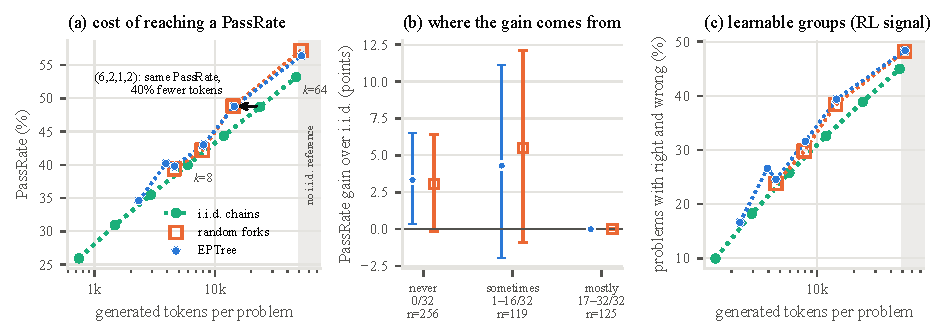
\includegraphics[width=\textwidth]{figures/task2_passrate.pdf}
\caption{Tree sampling vs.\ i.i.d.\ chains on 500 Omni-MATH problems.
(a)~PassRate (at least one correct response) against generated tokens.
(b)~Gain over i.i.d.\ chains at the same token budget, per problem with a 95\% bootstrap CI. The i.i.d.\ PassRate is interpolated log-linearly in tokens between neighbouring $k$. $(8,4,2,2)$ is omitted because it exceeds the 64-chain budget.}
\label{fig:task2-passrate}
\end{figure*}

\begin{table*}[t]
\centering\footnotesize
\setlength{\tabcolsep}{4.5pt}
\begin{tabular}{@{}lrrrrrrr@{}}
\toprule
$(M,N,L,T)$ & Leaves & Tokens & EPTree & Random & i.i.d.\ at same tokens & EPTree $-$ i.i.d.\ [95\% CI] & EPTree $-$ Random [95\% CI] \\
\midrule
(2,1,1,1) & 4 & 2.3k & 34.6 & -- & 34.0 & $+0.6$ [$-1.3$, $+2.6$] & -- \\
(2,3,1,1) & 8 & 3.9k & 40.2 & -- & 37.4 & $+2.8$ [$+0.6$, $+5.0$] & -- \\
(4,1,1,1) & 8 & 4.6k & 39.8 & 39.4 & 38.4 & $+1.4$ [$-0.6$, $+3.5$] & $+0.4$ [$-2.0$, $+2.8$] \\
(4,3,1,1) & 16 & 8.0k & 43.0 & 42.2 & 41.9 & $+1.1$ [$-0.9$, $+3.2$] & $+0.8$ [$-1.6$, $+3.4$] \\
(6,2,1,2) & 30 & 14.5k & 48.8 & 48.8 & 45.6 & $+3.2$ [$+1.0$, $+5.3$] & $\phantom{+}0.0$ [$-2.4$, $+2.4$] \\
(8,4,2,2) & 136 & 52.4k & 56.4 & 57.2 & -- & -- & $-0.8$ [$-3.2$, $+1.6$] \\
\bottomrule
\end{tabular}
\caption{PassRate (\%) of tree sampling on 500 Omni-MATH problems. Tokens are generated tokens per problem, counted once per shared prefix. The i.i.d.\ column is pass@$k$ at the same token budget. i.i.d.\ chains reach 44.4\% at 16 chains and 53.2\% at 64.}
\label{tab:task2}
\end{table*}

\paragraph{Trees beat i.i.d.\ sampling at the same cost.}
Every tree configuration lies above the i.i.d.\ curve (Figure~\ref{fig:task2-passrate}a). The gain at a matched token budget is $+0.6$ to $+3.3$ points, and significant for $(2,3,1,1)$ and $(6,2,1,2)$ (Figure~\ref{fig:task2-passrate}b, Table~\ref{tab:task2}). This replicates the paper's main inference result.

\paragraph{Where to fork matters little for PassRate.}
At identical $(M,N,L,T)$, entropy-guided and random forking differ by $+0.4$, $+0.8$, $0.0$ and $-0.8$ points, and every CI includes zero. The paper's differences ($+2.1$, $+1.0$) lie inside our intervals. In this setting the gain over i.i.d.\ sampling comes mostly from sharing prefixes, not from choosing the fork point.

\begin{figure}[t]
\centering
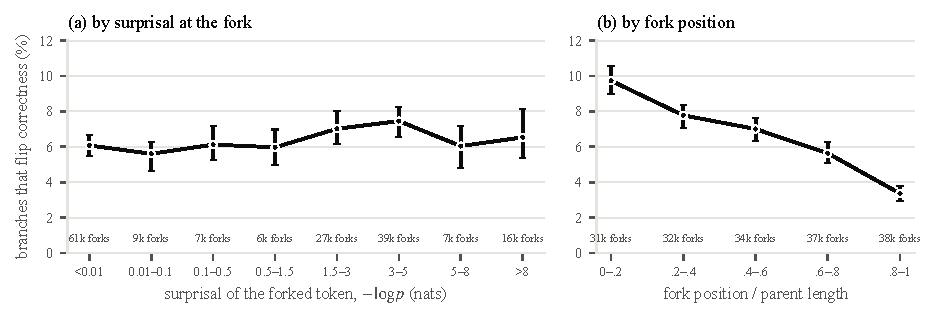
\includegraphics[width=\columnwidth]{figures/task2_forks.pdf}
\caption{Fork points of EPTree vs.\ random forking (four tree shapes run with both, 84k forks each).
(a)~Distribution of the surprisal of the token forked at.
(b)~Share of branches whose final answer, or whose correctness, differs from their parent's, per problem with a 95\% bootstrap CI.}
\label{fig:task2-forks}
\end{figure}

\paragraph{Surprisal finds uncertain tokens, rarely consequential ones.}
EPTree does fork where the model is uncertain: the forked token has a median surprisal of 3.56 nats, while 63\% of random forks land on near-certain tokens (Figure~\ref{fig:task2-forks}a). Its branches also end in a different final answer more often than random branches: 46.6\% vs.\ 42.6\%, paired difference $+4.0$ [$+3.2$, $+4.8$].

However, a branch changes correctness, the evidence that credit assignment needs, in only 7.0\% of cases for EPTree and 6.1\% for random forks ($+0.9$ [$+0.5$, $+1.3$]). Over 90\% of rollouts reproduce their parent's outcome. Fork positions are spread across the response (mean relative position 0.50), and the most frequent fork tokens are function words and \LaTeX{} delimiters.

This is the gap our method targets. Surprisal is a reasonable exploration signal, but most of a fixed budget spent on it yields no counterfactual evidence. Phase~II therefore spends the reserved $k$ rollouts only on states that are both novel and consequential.

\subsection{RL baselines}
\label{sec:rl}

\paragraph{Short runs.}
With 40 steps at the paper's learning rate, none of the three methods changes the model measurably. On greedy MATH500, for example, step-40 checkpoints score 74.4--75.4 against the base model's 74.6, and every difference across the three benchmarks is within noise. We therefore ran 150 steps with a higher learning rate ($5{\times}10^{-6}$).

\begin{figure*}[t]
\centering
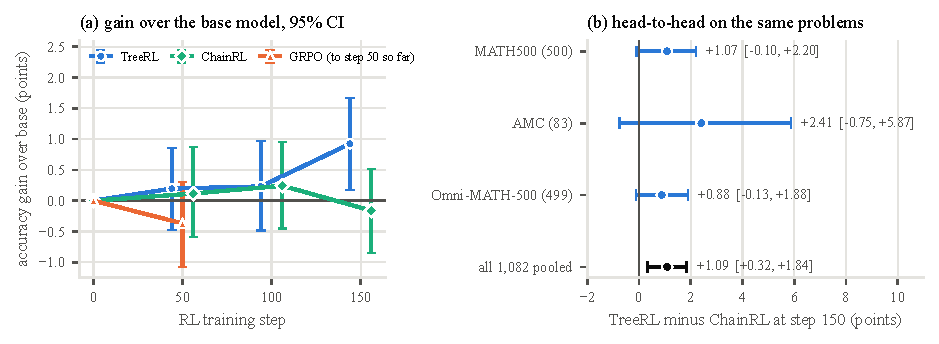
\includegraphics[width=\textwidth]{figures/rl_results.pdf}
\caption{RL with Qwen2.5-Math-1.5B-Instruct: 150 steps, 8 problems $\times$ 8 trained responses per step. Accuracy is mean@8 on the same 1{,}082 test problems, with paired bootstrap 95\% CIs.
(a)~Gain over the base model during training. GRPO is evaluated up to step 50 so far.
(b)~TreeRL minus ChainRL at step 150, per benchmark and pooled.}
\label{fig:rl}
\end{figure*}

\begin{table}[t]
\centering\small
\setlength{\tabcolsep}{4pt}
\begin{tabular}{@{}lrrrrr@{}}
\toprule
 & MATH500 & AMC & Omni & Pooled & Mean \\
\midrule
Base & 73.95 & 45.03 & 26.68 & 49.93 & 48.55 \\
ChainRL & 73.83 & 45.78 & 26.33 & 49.77 & 48.65 \\
GRPO & \multicolumn{5}{c}{in progress} \\
TreeRL & \textbf{74.90} & \textbf{48.19} & \textbf{27.20} & \textbf{50.85} & \textbf{50.10} \\
\midrule
\multicolumn{6}{@{}l}{TreeRL $-$ ChainRL, pooled: $+1.09$ [$+0.32$, $+1.84$]} \\
\bottomrule
\end{tabular}
\caption{Mean@8 accuracy (\%) at step 150 of the long runs. Pooled: over all 1{,}082 problems. Mean: unweighted mean of the three benchmarks, as the paper reports.}
\label{tab:rl}
\end{table}

\paragraph{Long runs.}
TreeRL and ChainRL are indistinguishable at steps 50 and 100 (Figure~\ref{fig:rl}a). By step 150, TreeRL improves over the base model by $+0.92$ points [$+0.17$, $+1.66$], while ChainRL stays at the base level ($-0.16$ [$-0.85$, $+0.52$]).

Head-to-head on the same problems, TreeRL leads ChainRL by $+1.09$ [$+0.32$, $+1.84$] (Figure~\ref{fig:rl}b, Table~\ref{tab:rl}). It is ahead on every benchmark: MATH500 $+1.07$, AMC $+2.41$, Omni-MATH-500 $+0.88$. Excluding the 15 test problems that overlap the training data gives $+1.04$ [$+0.27$, $+1.79$].

The pattern matches the paper, where both methods track each other early and TreeRL pulls ahead after about 100 of $\sim$300 steps. The size of the gap is close to the paper's for an already strong policy: $+1.3$ for R1-Distill-Qwen-7B.

\paragraph{Caveats.}
\begin{itemize}
\item Each method was trained once, so run-to-run variance is not yet measured.
\item The methods are matched on trained responses, not on generated tokens. Our TreeRL generates about $2.4\times$ more tokens than ChainRL, whereas the paper matches generated tokens.
\item Our budget (150 steps $\times$ 64 responses) is roughly 1/15 of the paper's. The base policy, already tuned for math by its developers, leaves little headroom on MATH-level problems.
\item The GRPO baseline has finished 50 of its 150 steps.
\end{itemize}
